\documentclass{standalone}
\usepackage{tikz}
\usetikzlibrary{patterns}
\usepackage{pgfplots}
\begin{document}%
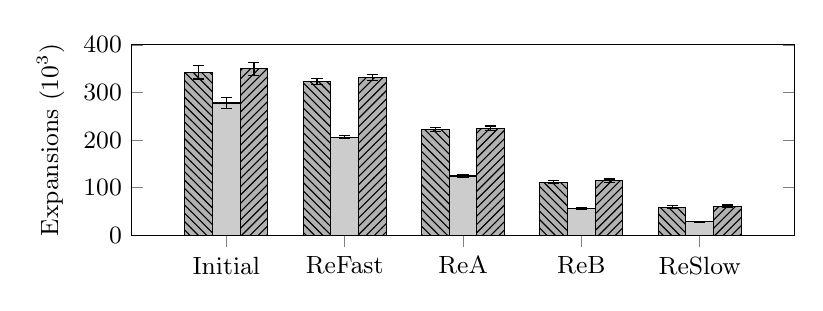
\begin{tikzpicture}[font=\small]

% this stats are currently manually computed
% from results of experiment: Makefile.incbi-road-ne


\begin{axis}[
   ybar=0pt,
   %bar width=0.20cm,
   enlarge x limits=0.2,
   width=10cm, height=4cm,
   ymin=0,
   ylabel={Expansions ($10^3$)},
   xlabel near ticks,
   ylabel near ticks,
   xtick=data,
   symbolic x coords={Initial,ReFast,ReA,ReB,ReSlow},
   xtick pos=left,
   ]

% lpastar
\addplot+[black,fill=black!30,
   postaction={pattern=north west lines},
   error bars/.cd,y dir=both,y explicit]
coordinates
{
   (Initial,342.307755) +- (14.056335,14.056335)
   (ReFast,323.0747175) +- (5.942065727060889,5.942065727060889) % pblock = 0.0010
   (ReA,222.00896138888889) +- (4.9069293742642285,4.9069293742642285) % pblock = 0.0005
   (ReB,111.56027138888888) +- (3.3797460326690284,3.3797460326690284) % pblock = 0.0002
   (ReSlow,59.14850027777778) +- (2.442949291075538,2.442949291075538) % pblock = 0.0001
};

% incbi
\addplot+[black,fill=black!20,
   error bars/.cd,y dir=both,y explicit]
coordinates
{
   (Initial,277.9990225) +- (10.87699206318198,10.87699206318198)
   (ReFast,206.19699694444446) +- (3.766655746404173,3.766655746404173) % pblock = 0.0010
   (ReA,124.36986944444444) +- (2.648126726146959,2.648126726146959) % pblock = 0.0005
   (ReB,55.84239638888889) +- (1.5884328609708211,1.5884328609708211) % pblock = 0.0002
   (ReSlow,28.027845833333333) +- (1.074324688281415,1.074324688281415) % pblock = 0.0001
};

% rlpastar
\addplot+[black,fill=black!30,
   postaction={pattern=north east lines},
   error bars/.cd,y dir=both,y explicit]
coordinates
{
   (Initial,350.20625) +- (13.705055946042474,13.705055946042474)
   (ReFast,331.56562555555557) +- (5.9194884547474185,5.9194884547474185) % pblock = 0.0010
   (ReA,224.65325444444444) +- (4.8653007345139,4.8653007345139) % pblock = 0.0005
   (ReB,114.67884694444445) +- (3.5342402251294957,3.5342402251294957) % pblock = 0.0002
   (ReSlow,60.82335083333333) +- (2.5823248997652113,2.5823248997652113) % pblock = 0.0001
};

\end{axis}

\end{tikzpicture}%
\end{document}
